\documentclass[12pt, twoside]{article}
\usepackage[letterpaper, margin=1in, headsep=0.5in]{geometry}
\usepackage[english]{babel}
\usepackage[utf8]{inputenc}
\usepackage{amsmath}
\usepackage{amsfonts}
\usepackage{amssymb}
\usepackage{tikz}
\usetikzlibrary{quotes, angles}
\usepackage{graphicx}
\usepackage{enumitem}
\usepackage{multicol}

\newif\ifmeta
\metatrue %print standards and topics tags

\title{Regents Geometry}
\author{Chris Huson}
\date{September 2020}

\usepackage{fancyhdr}
\pagestyle{fancy}
\fancyhf{}
\renewcommand{\headrulewidth}{0pt} % disable the underline of the header
\raggedbottom


\fancyhead[LE]{\thepage}
\fancyhead[RO]{\thepage \\ Name: \hspace{4cm} \,\\}
\fancyhead[LO]{BECA / Dr. Huson / Geometry 08-Area+volume\\* pset ID: 129}

\begin{document}

\subsubsection*{8-1DN-Circle-trajectories}
\begin{enumerate}
\subsubsection*{Sketch the situation on the axes. Mark important values. Do NOT solve!}
 
\item The line represented by $2y=x+8$ is dilated by a scale factor of $k$ centered at the origin, such that the image of the line has an equation of $\displaystyle y-\frac{1}{2}x=2$. What is the scale factor?
  \begin{center}
    \begin{tikzpicture}[scale=.48]
      \draw [thick, <->] (-10.4,0) -- (10.4,0) node [right] {$x$};
      \draw [thick, <->] (0,-10.4)--(0,10.4) node [above] {$y$};  
  \end{tikzpicture}
  \end{center}

\newpage
\subsubsection*{Vocabulary situations: show circle with parts}
    
\item Given the circle, points, and line segments depicted below, circle whether each statement is true or false.
  (Circle with chords, secant, radius, diameter, arc, center, circumference, semicircle, tangent, perpendicular situations)
  
\item Triangle vocabulary: vertex, side, hypotenuse, acute, obtuse, perpendicular, median, altitude, perpendicular bisector
  
\item Situations with right triangle hypotenuses as circle radii.

\item Use the tangent function to determine the measure of the central angle $\theta$.
  
\item A regular pentagon is inscribed in a circle as shown below. What is the measure of the central angle between two consecutive vertices, $m\angle AOB$?
  
\subsubsection*{Area and volume formula applications}

\item Formulas for the area and circumference of circles:\\
  $A=\pi r^2$\\
  $C=\pi D = 2\pi r$
    \begin{enumerate}
    \item Find the area of a circle with radius 4 cm.
    \item Find the radius of a circle having an area of $25 \pi$.
    \end{enumerate}

\newpage
\subsubsection*{Equation of a circle algebra competencies} 

\item Expand each binomial-squared expression to the form $ax^2+bx+c$.
  \begin{multicols}{2}
  \begin{enumerate}[itemsep=2cm]
    \item $(x+3)^2$
    \item $(x+2)^2$ 
    \item $(x+5)^2$ 
    \item $(x+7)^2$ 
  \end{enumerate}
  \end{multicols}\vspace{2cm}

\item Factor each trinomial as a binomial squared.
  \begin{multicols}{2}
    \begin{enumerate}[itemsep=2cm]
      \item $x^2+2x+1$ 
      \item $x^2+8x+16$
      \item $x^2+12x+36$ 
      \item $x^2+16x+64$ 
    \end{enumerate}
    \end{multicols}\vspace{2cm}

\item Simplify each radical.
  \begin{multicols}{2}
    \begin{enumerate}[itemsep=2cm]
      \item $\sqrt{50}$ 
      \item $\sqrt{18}$
      \item $\sqrt{27}$ 
      \item $\sqrt{24}$ 
    \end{enumerate}
    \end{multicols}\vspace{2cm}
    
\item What are the coordinates of the center and the length of the radius of the circle whose equation is $x^2 + y^2 = 8x -6y +39$?

\newpage
\item On the set of axes below, $\overline{AB}$ is dilated with a scale factor of $\frac{5}{2}$ centered at point $P$.
  \begin{multicols}{2}
  Which of the following is/are true:
  \begin{enumerate}
  \item T \quad F \quad $\overline{AP} \cong \overline{AA'}$
  \item T \quad F \quad $\overline{AB} \parallel \overline{A'B'}$
  \item T \quad F \quad $AB = A'B'$
  \item T \quad F \quad $\displaystyle \frac{5}{2} (A'B') = AB$
  \end{enumerate}
  \begin{flushright}
    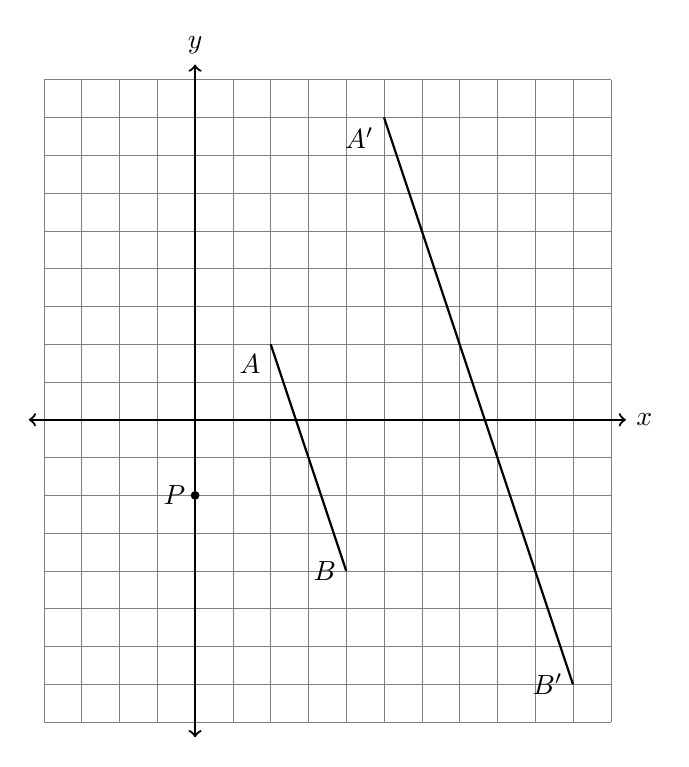
\begin{tikzpicture}[scale=.48]
      \draw [help lines] (-4,-8) grid (11,9);
      \draw [thick, <->] (-4.4,0) -- (11.4,0) node [right] {$x$};
      \draw [thick, <->] (0,-8.4)--(0,9.4) node [above] {$y$};  
      \draw [thick]
        (2,2) node[below left] {$A$}--
        (4,-4) node[left] {$B$};
      \draw [thick]
        (5,8) node[below left] {$A'$}--
        (10,-7) node[left] {$B'$};
      \draw [fill] (0,-2) circle [radius=0.1]node[left]{$P$};
  \end{tikzpicture}
  \end{flushright}
  \end{multicols}

\item The coordinates of the vertices of parallelogram $CDEH$ are $C(-5,5)$, $D(2,5)$, $E(-1,-1)$, and $H(-8,-1)$. What are the coordinates of $P$, the point of intersection of diagonals $\overline{CE}$ and $\overline{DH}$? \\[0.25cm] (scaffold to graph on exam stationary)
  \begin{center}
    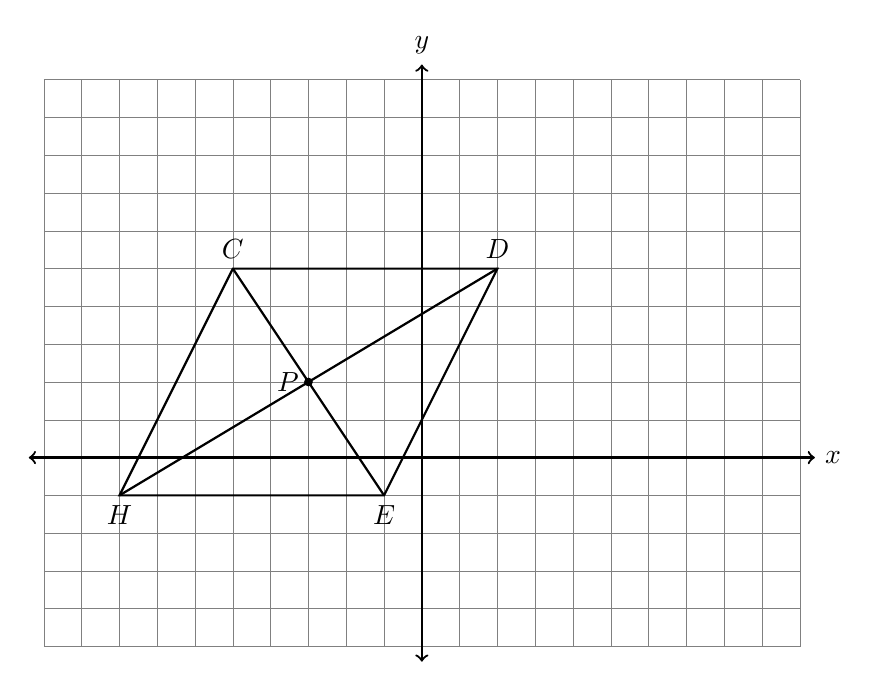
\begin{tikzpicture}[scale=.48]
      \draw [help lines] (-10,-5) grid (10,10);
      \draw [thick, <->] (-10.4,0) -- (10.4,0) node [right] {$x$};
      \draw [thick, <->] (0,-5.4)--(0,10.4) node [above] {$y$};  
      \draw [thick]
        (-5,5) node[above] {$C$}--
        (2,5) node[above] {$D$}--
        (-1,-1) node[below] {$E$}--
        (-8,-1) node[below] {$H$}--cycle;
      \draw [thick]
        (-5,5)--
        (-1,-1);
      \draw [thick]
        (2,5)--
        (-8,-1);
      \draw [fill] (-3,2) circle [radius=0.1]node[left]{$P$};
  \end{tikzpicture}
  \end{center}

\end{enumerate}
\end{document}